
\documentclass{article}
\usepackage{graphicx}
%\usepackage{feynmp}
\usepackage{subfigure}
\graphicspath{{figs/}}

\title{Deep Learning Notes}

\author{Peter Thompson}

\begin{document}

\section{random notes}
Don't use sigmoid as an activation function. Tanh is generally superior, as it has a mean of zero (sigmoid has a mean of 0.5). Nonzero mean can make training more difficult in subsequent layers. Tanh has a mean of zero. May want a sigmoid as a final activation function (that is, in the output layer) when doing a binary classification problem.

relu is generally good.



\section{notation}
\section{logstic loss}

loss function is the loss/error associated with a single training example
Cost function is the loss computed over all examples

logistic loss

Think of $\hat{y}$ as the conditional probability $\hat{y}(x) = P(y=1|x)$. The probability $y=0$ is then $P(y=0|x) = 1 - \hat{y}$. These two outcomes can be summarised as
\begin{equation}
P(y|x) = \hat{y}^y(1-\hat{y})^{(1-y)}
\end{equation}
The above is for a single example. The likelihood (of parameters) for a given training set would be obtained from the product $\prod_i P(y_i|x_i)$, where $\hat(y)_i$ is a function of $x_i$.

The expression for logistic loss can then be obtained from the negative log likelihood of $P(y|x)$ above
\begin{equation}
L = \sum_i  (y_i-1) ln(1 - \hat{y}_i) - y_i ln(\hat{y}_i)
\end{equation}
The log of the product reduces to a sum over logs.



\section{activation functions and their derivatives}


\subsection{sigmoid}
The sigmoid function (or logit function) and its derivative are given by
\begin{eqnarray*}
\sigma(x) & = &\frac{1}{1 - e^{-x}} \\
\frac{d\sigma(x)}{dx} & = & \sigma(x)(1 - \sigma(x)) \\
\end{eqnarray*}

these are plotted below
\begin{figure}[tb]
\begin{centering}
\subfigure{
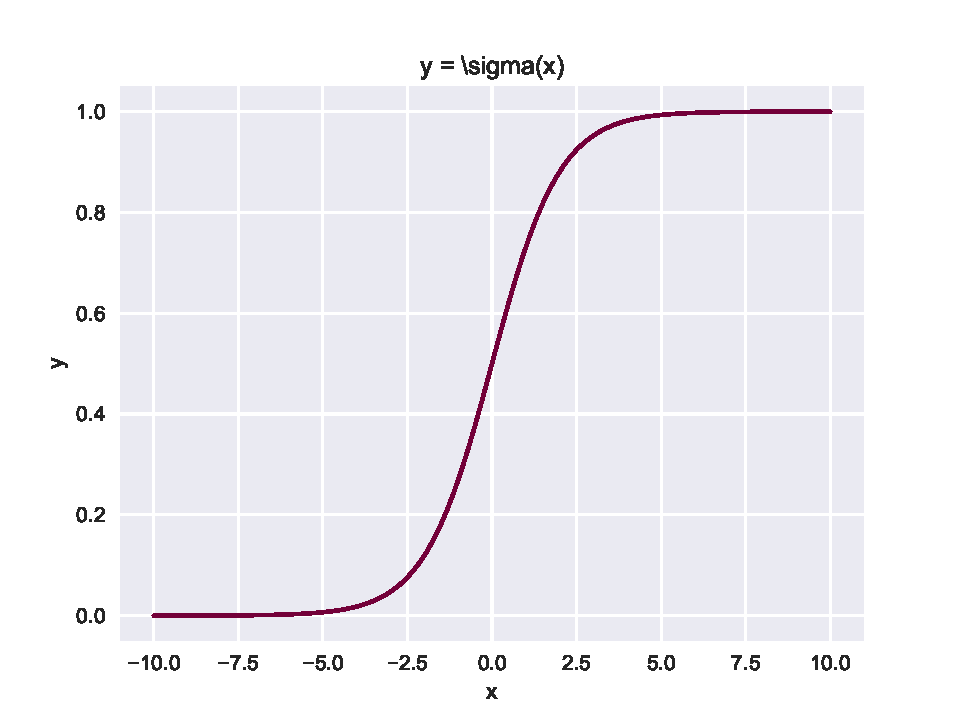
\includegraphics[width=0.45\linewidth,angle=0]{sigmoid.pdf}
% \caption{sigmoid activation function}
}
\subfigure{
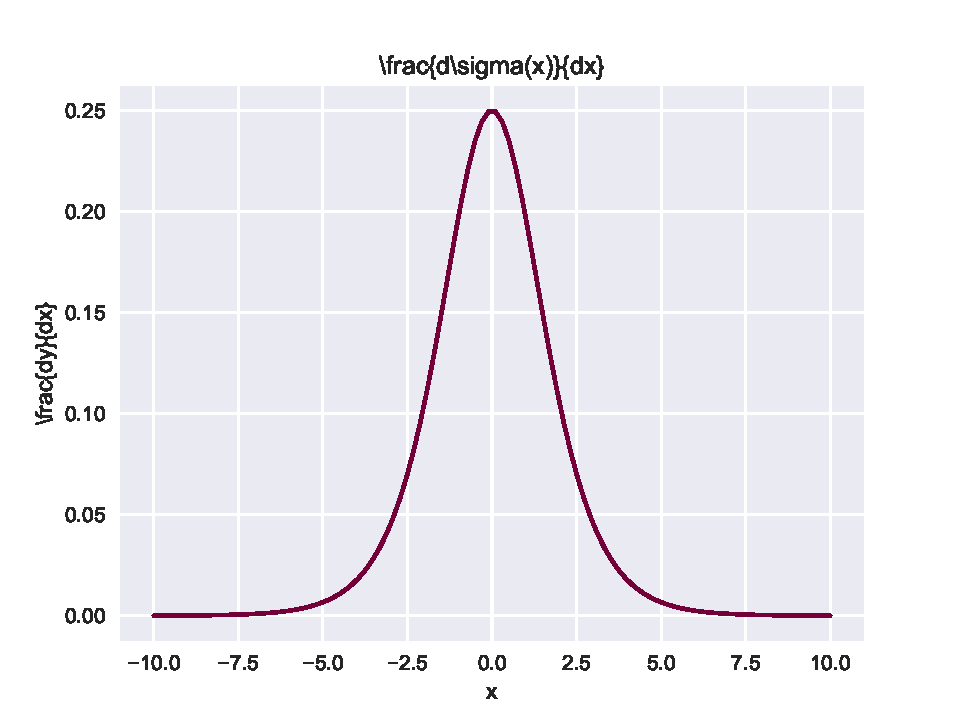
\includegraphics[width=0.45\linewidth,angle=0]{sigmoid_derivative.pdf}
% \caption{sigmoid derivative}
}
\end{centering}
\end{figure}

\subsection{tanh}
The tanh function (sinh/cosh) and its derivative are given by
\begin{eqnarray*}
\mathrm{tanh}(x) & = &\frac{e^x\,-\, e^{-x}}{e^x\,+\, e^{-x}} \\
\frac{d\sigma(x)}{dx} & = & 1 - \mathrm{tanh}^2(x) 
\end{eqnarray*}

these are plotted below
\begin{figure}[tb]
\begin{centering}
\subfigure{
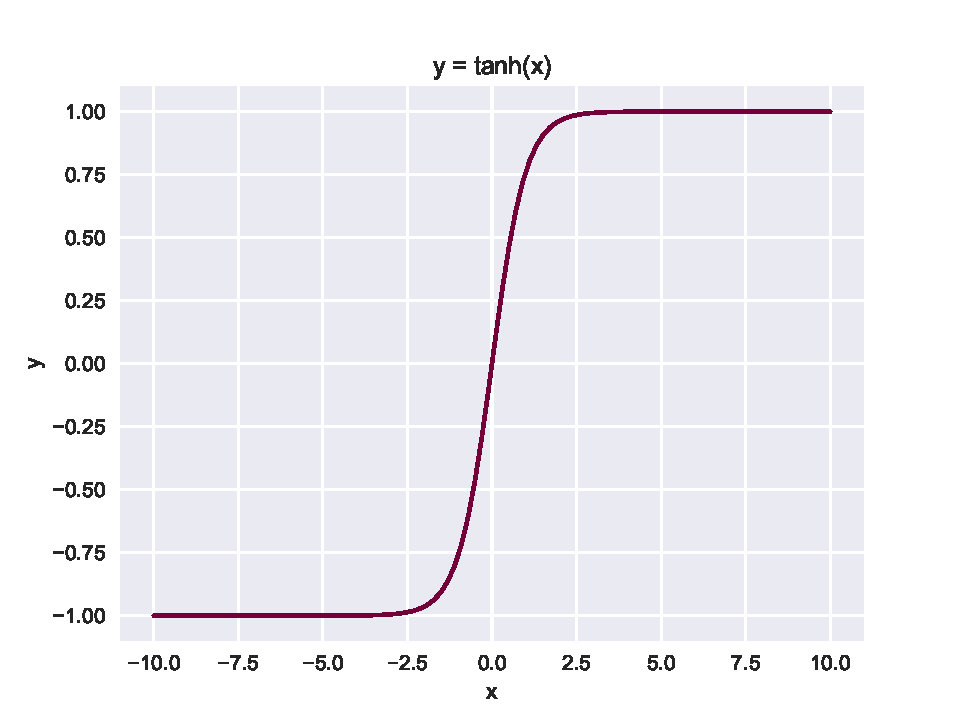
\includegraphics[width=0.45\linewidth,angle=0]{tanh.pdf}
% \caption{tanh activation function}
}
\subfigure{
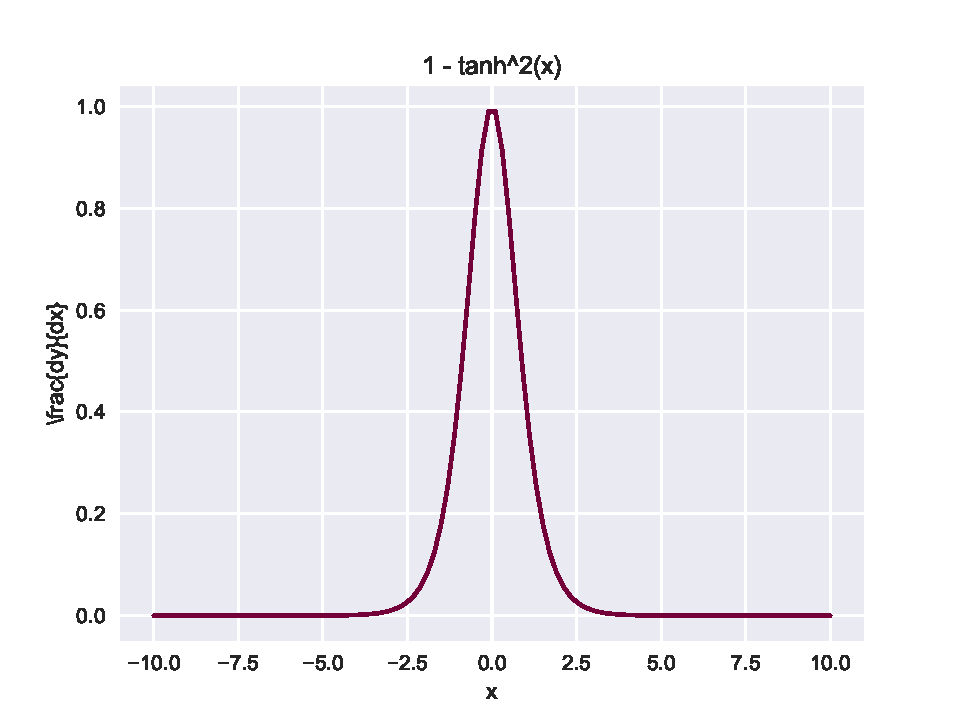
\includegraphics[width=0.45\linewidth,angle=0]{tanh_derivative.pdf}
% \caption{tanh derivative}
}
\end{centering}
\end{figure}

\subsection{ReLu}
rectified linear unit
\subsection{leaky ReLu}
Gradient saturation and such
\end{document}

